\documentclass[11pt,titlepage]{article}
%\usepackage[notref]{showkeys}
\usepackage[reqno]{amsmath}
\usepackage{natbib}
\usepackage{amssymb}
\usepackage{epsfig}
\usepackage{comment}
\usepackage{url}
\usepackage[all]{xy}        
\usepackage{dcolumn}
\newcolumntype{.}{D{.}{.}{-1}}
\newcolumntype{d}[1]{D{.}{.}{#1}}
\usepackage{threeparttable,booktabs}
\usepackage{times}
\usepackage{vmargin}
\setpapersize{USletter}
\topmargin=0in

% Shortcuts
\renewcommand{\P}{\text{P}}
\newcommand{\MC}{\multicolumn}
\usepackage{calc}
\newcounter{hours}\newcounter{minutes}
\newcommand{\printtime}{%
  \setcounter{hours}{\time/60}%
  \setcounter{minutes}{\time-\value{hours}*60}%
  \thehours :\theminutes}
%
\title{The Balance Test Fallacy\thanks{Our thanks to Dan Carpenter and
    Jeff Koch for data, and the National Institutes of Aging (P01
    AG17625-01) and the National Science Foundation (SES-0318275,
    IIS-9874747) for research support.  Software to implement the
    methods in this paper is available at
    \texttt{http://GKing.Harvard.edu/matchit}.}}

\author{Kosuke Imai,\thanks{Assistant Professor, Department of
    Politics, Princeton University (Corwin Hall 041, Department of
    Politics, Princeton University, Princeton NJ 08544, USA;
    \texttt{http://Imai.Princeton.Edu}, \texttt{kimai@Princeton.Edu},
    (609) 258-6601).}
%\and %
  Gary King,\thanks{David Florence Professor of Government, Harvard
    University (Institute for Quantitative Social Science, Harvard
    University, 1737 Cambridge St., Cambridge MA 02138;
    \texttt{http://GKing.Harvard.Edu}, \texttt{King@Harvard.Edu},
    (617) 495-2027).}
%\and %
Elizabeth A. Stuart\thanks{Researcher, Mathematica Policy Research,
  Inc.\, Ph.D.\, Department of Statistics, Harvard University.
  (600 Maryland Ave., SW, Suite 550,  Washington, DC, 20024, USA;
  \texttt{http://people.iq.harvard.edu/$\sim$estuart/},
  \texttt{Stuart@Stat.Harvard.Edu}).}}

\date{\today\ (\printtime)} 

\begin{document}\maketitle

A good matching procedure reduces bias by increasing balance, does not
increase the variance much, and prevents inducing new biases by
matching only based on $X$ without consulting $y$ until the analysis
stage.  We assume matching is based only on $X$, and checking the
number of observations remaining after matching is easy.  Thus, the
main issue we address in this section and the next is how to evaluate
balance.  Conceptually, verifying balance involves checking whether
(\ref{balance}), $\tilde p(X|t=1)=\tilde p(X|t=0)$, holds.  One way to
think about this process is to imagine, for all the variables in $X$,
forming a multidimensional histogram for all the treated units and
comparing it to another multidimensional histogram of all the control
units.  Because of the curse of dimensionality, multidimensional
histograms with more than a few covariates tend to be very coarse or
have many empty bins, and so using them to estimate the two underlying
probability densities in (\ref{balance}) will ordinarily be very
difficult without access to an extraordinary number of observations.
Thus researchers usually examine various low dimensional summaries
instead.  If a low dimensional summary differs between the treated and
control groups then (\ref{balance}) does not hold.  The risk of course
is that even if the treatment and control groups match according to
some low dimensional summaries, we still cannot be certain that
(\ref{balance}) holds since it is a multivariate concept, and so using
several different checks is always a good idea.

Here we describe what we call the balance test fallacy, which
unfortunately characterizes most applications of matching in most
fields.  The critical misunderstood point is that balance is a
characteristic of the observed sample, not some hypothetical
population.  The idea that hypothesis tests are useful for checking
balance is therefore incorrect, and t-statistics below 2 and p-values
above 0.05 have no special relevance for assessing balance.

The fallacy has several serious implications.  First, balance tests do
not provide levels below which imbalance can be ignored: The closer
the two observed treatment and control groups in the sample, the
better.  Even though we might use a hypothetical population that
generates the observed $X$ to think about concepts like common
support, it is the observed sample that is relevant for generating
balance.  To see this, consider in assessing the effect of some
treatment whether we want the treatment and control groups to be
identical, or whether we should be willing to risk them being slightly
different.  The problem that has been ignored is that if the
difference, no matter how small, occurs for a variable that happens to
have a large enough effect on $Y$, then this tiny or ``insignificant''
imbalance can translate into a large bias and/or inefficiency in our
causal estimates.

The balance test fallacy has led hypothesis tests to be used
extensively in applications of matching.  Most commonly, tables of
t-tests for differences in means are offered as evidence that balance
has been ``achieved''.  This is unfortunate since a better balanced
sample, that would reduce bias even further, can often be found.  But
even more importantly, hypothesis tests not only can cause one to stop
too soon, but they can be highly misleading even when using them as
objective functions to optimize.  In particular, pruning too many
observations reduces the statistical power of a hypothesis test (i.e., the
probability of rejecting the null hypothesis) and thus affects the
test, even if this pruning does not improve balance at all.

\begin{figure}[t] 
 \begin{center}
   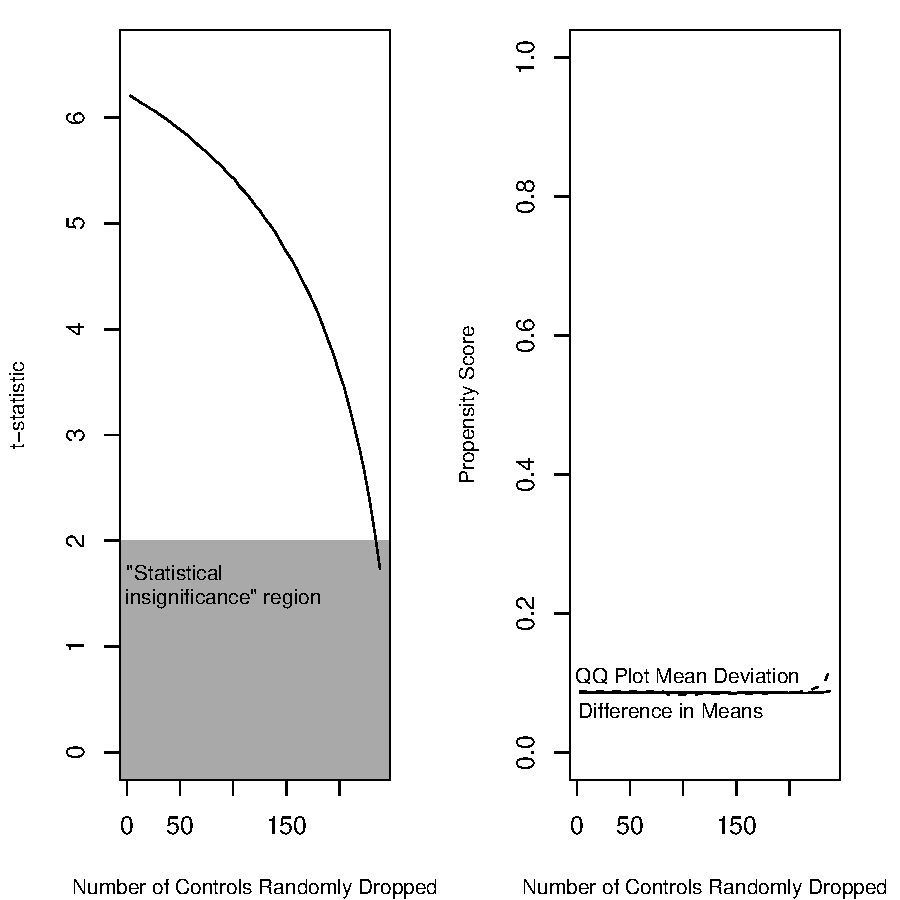
\includegraphics[height=4in]{figs/TStatPlotPscore.pdf}
  \end{center}
  \vspace{-0.275in}
  \caption{Dangers in relying on t-statistics as measure of balance.
    The solid lines in both graphs indicate the average value of a
    measure of balance when a given number of control units are
    randomly dropped from the data set (out of a total of 245).  With
    larger numbers of control units dropped (i.e., smaller numbers of
    control units in the resulting sample), the t-statistic gets
    closer to 0, falsely indicating reductions in balance with the
    smaller resulting sample sizes, even though true balance does not
    vary systematically across the data sets.}
  \label{f:tstat}
\end{figure}

To illustrate the dangers of using hypothesis tests to assess balance,
we created a sequence of matched data sets by \emph{randomly} pruning
increasing numbers of control group observations (from the real data
set we analyze in Section~\ref{s:carp}).  Random matching procedures
have no systematic effect on balance.  Yet, the left graph in
Figure~\ref{f:tstat}, which plots the number of observations dropped
(plotted horizontally) by the t-statistic (plotted vertically), shows
that the t-statistic falsely indicates a dramatic improvement in
balance.  The area where the t-statistic falls below 2 is normally
(but incorrectly) identified as ``insignificant imbalance,'' and
clearly the t-statistic drops into this area (colored grey in the
figure) only because of the sample size and regardless of the fact
that the balance does not differ systematically as more observations
are dropped.  In fact, since hypothesis test are driven in part by
factors other than balance, they are not even monotonic functions of
balance: the t-test can get apparently better while balance gets
worse, or vice versa.\footnote{To see this, consider the commonly-used
  two sample $t$-test statistic with unknown and unequal variances,
  which can be written as, $\sqrt{n}(\overline{X}_t-\overline{X}_c)/
  \sqrt{\frac{s^2_t}{r} + \frac{s^2_c}{1-r}}$ where
  $s^2_t=\sum_{i=1}^n t_i(X_i - \overline{X}_t)^2/(n_t-1)$,
  $s^2_c=\sum_{i=1}^n (1-t_i)(X_i - \overline{X}_t)^2/(n_c-1)$, $n_t$
  and $n_c$ are the sample size for the treatment and control groups,
  and $r=n_t/n$.  Hence, the difference in sample means as a measure
  of balance is thus distorted in the t-test due to the three factors:
  the total number of remaining observations $n$, the ratio of
  remaining treated units to the total number of remaining
  observations $r$, and the variance of $X$ for the remaining treated
  and control units, $s_t^2$ and $s_c^2$ respectively.}

\baselineskip=0.637\baselineskip 
\bibliographystyle{apsr}
\bibliography{gk,gkpubs}

\end{document}
